\label{chap:context}
\section{General problem}
\subsection{Formulation}
Generic formulation of the object detection problem
\subsection{Implementation issues}
What issues an implementor could face when trying to implement object detection in large images
\subsection{Related works}
What solutions are usually presented in the litterature to solve those problems (shallow overview as this is a wide topic) 
\section{Cytology}
According to the Collins dictionary, cytology is "\textit{the study of plant and animal cells, including their structure, function and formation}" \cite{collins-cytology}. 

Digitization

\subsection{Thyroid cytology and nodule malignancy}
\label{ssec:intro_thyroid_case}
Nodules are growths than can develop in the thyroid. Usually, they are benign but in some cases they can be a sign of a cancer (?? give prevalence, probabilities ??). Therefore, patients presenting those nodules are subjected to a range of medical examinations. One of the most important step in those examination is the fine needle aspiration biopsy (FNAB) \cite{bomeli2010evaluation}. It consists in taking a sample of tissues directly inside the nodule mass. Those takings are then stained and examined under a microscope by a physician. Especially, the nodule malignity is confirmed by the presence of some specific features such as intra-nuclear inclusions or proliferative architectural patterns. Example of stained takings are shown in Figures \ref{fig:intro_inclu_ex} and \ref{fig:intro_pattern_ex}. In the former are shown cells with inclusion which are recognizable because of the typical brighter circular area inside the cell. In the latter are shown architectural patterns. Especially, proliferative patterns are shown in Figure \ref{sfig:prolif_patterns} while non-proliferative ones are shown in \ref{sfig:norm_patterns}. 

\begin{figure}
	\center
	\subfigure{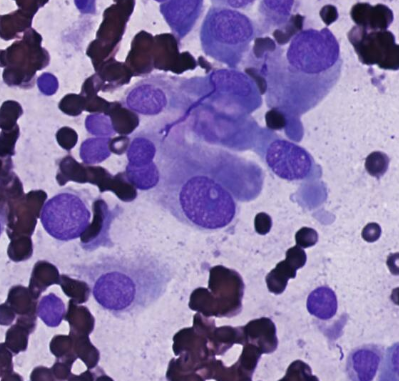
\includegraphics[scale=0.5]{image/inclusion_1.png}}
	\subfigure{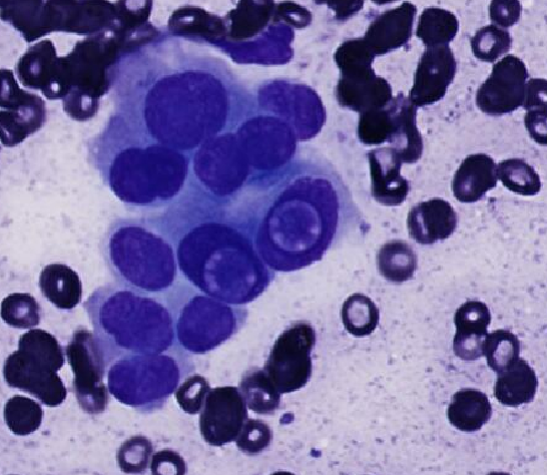
\includegraphics[scale=0.5]{image/inclusion_2.png}}
	\caption{Cells with inclusion}
	\label{fig:intro_inclu_ex}
\end{figure}

\begin{figure}
	\center
	\subfigure[Proliferative]{
		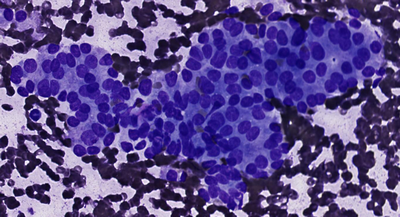
\includegraphics[scale=0.5]{image/prolif_pattern_1.png}
		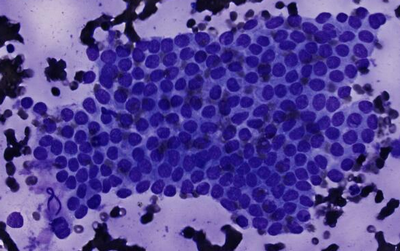
\includegraphics[scale=0.5]{image/prolif_pattern_2.png}
		\label{sfig:prolif_patterns}
	} \\
	\subfigure[Non-proliferative]{
		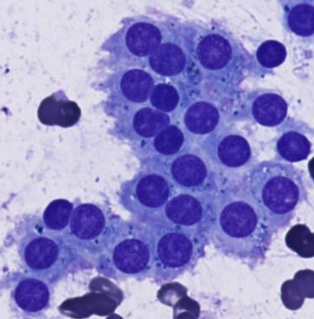
\includegraphics[scale=0.5]{image/normal_pattern_1.png}
		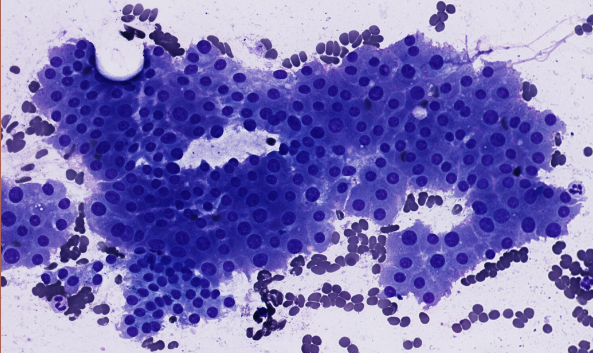
\includegraphics[scale=0.5]{image/normal_pattern_2.png}
		\label{sfig:norm_patterns}
	}
	\caption{Stained thyroid takings - architectural patterns}
	\label{fig:intro_pattern_ex}
\end{figure}



In the context of the Cytomine project, whole-slide 